\section{Graphical Editor Design} \label{sec:architecture}
Similar to the existing application the graphical editor is written in the Typescript\footnotemark\ language on top of the Angular framework \cite{ang&05}. \footnotetext{\url{https://www.typescriptlang.org/}}
Angular is a front end framework consisting of several libraries and utility programs that aid in the development of web applications.

The editor implements the \emph{model-view-controller} (MVC) design pattern \cite{Gamma&95}.
This emphasizes the separation of data of the application from how its represented graphically.
It allows the data of the model to be represented by multiple views.
A specific example of two views that share the same data are the project and canvas views, shown earlier in Figure~\ref{fig:scenario_editor_overview}.

\begin{figure}[H]
\centering
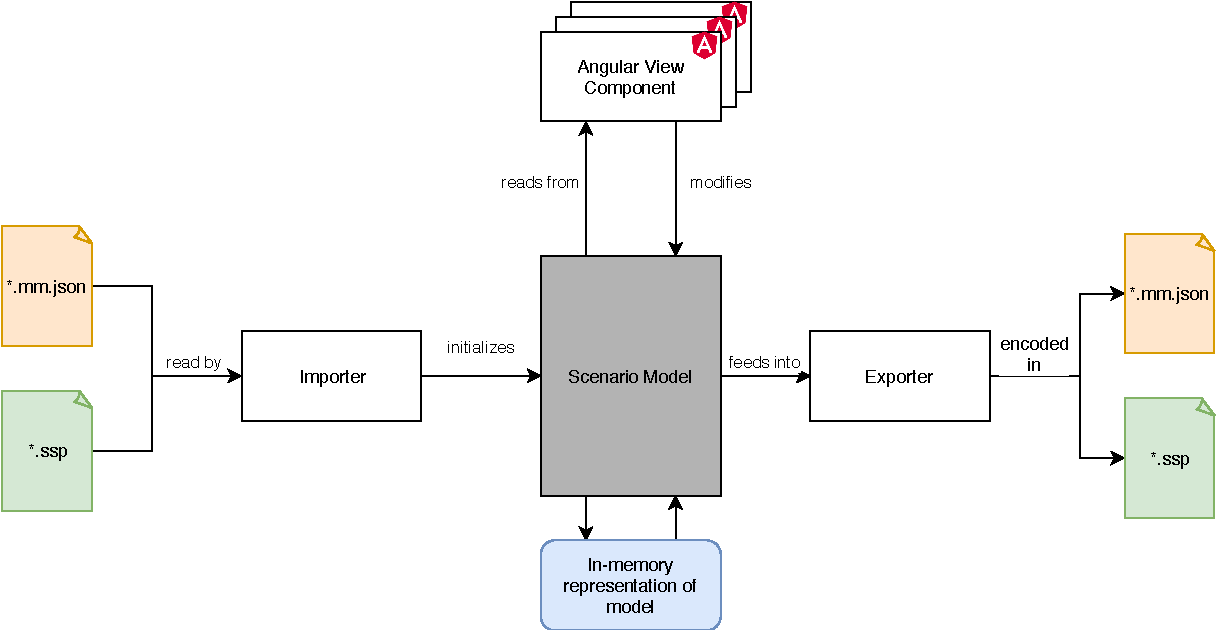
\includegraphics[width=\columnwidth]{Images/architecture_serialization.pdf}
\caption{Flow importing and exporting multi-models and SSPs}
\label{fig:architecture_serialization}
\end{figure}


A conceptual view of the architecture can be seen on Figure~\ref{fig:architecture_serialization}.
Starting from the left we see that a co-simulation scenario can be imported from a file encoded as either the current multi model format or the SSP format. 
The file is parsed and used to instantiate an in-memory representation of the scenario referred to as the \emph{scenario model}. 
The model has several uses. It provides an abstraction of the underlying model to components such as the editor.
The editor reads and generates a graphical representation of the model.
Conversely, changes to the scenario made through the editor are propagated back to the model.
Finally, the model may be exported to a format suitable for exchange, such as multi-model or SSP.

\subsection{Rendering of components}
The canvas-view is built on top of the javascript library mxGraph\footnote{\url{https://github.com/jgraph/mxgraph}}.
It provides the functionality of creating interactive graphs, creating connectors, undo-redo, automatic layout and much more.

\subsection{Modules}
Specifically the implementations consists of several components, referred to as a \emph{Modules} within the context of Angular\footnote{\url{https://angular.io/guide/architecture-modules}}.
A module is a collection of components and services which provide a coherent set of functionality to the application. In this setting the work presented in this paper naturally needs to fit into the recently developed cloud version of the INTO-CPS Application \cite{Rasmussen&19}.

To facilitate version management the modules are published on NPM under the namespace \emph{@into-cps}.
The concrete packages are listed below:
\begin{itemize}[\label={}]
\item \emph{@into-cps/graphical-editor}
\item \emph{@into-cps/scenario-model}
\item \emph{@into-cps/model-serialization}
\end{itemize}
